%%%%%%%%%%%%%%%%%%%%%%%%%%%%%%%%%%%%%%%%%%%%%%%%%%%%%%%%%%%%%%%%%%%%%%%%%%%%%%%%
%2345678901234567890123456789012345678901234567890123456789012345678901234567890
%        1         2         3         4         5         6         7         8

\documentclass[letterpaper, 10 pt, conference]{ieeeconf}  % Comment this line out
                                                          % if you need a4paper
%\documentclass[a4paper, 10pt, conference]{ieeeconf}      % Use this line for a4
                                                          % paper

\IEEEoverridecommandlockouts                              % This command is only
                                                          % needed if you want to
                                                          % use the \thanks command
\overrideIEEEmargins
% See the \addtolength command later in the file to balance the column lengths
% on the last page of the document



% The following packages can be found on http:\\www.ctan.org
\usepackage{graphics} % for pdf, bitmapped graphics files
%\usepackage{epsfig} % for postscript graphics files
%\usepackage{mathptmx} % assumes new font selection scheme installed
%\usepackage{times} % assumes new font selection scheme installed
\usepackage{amsmath} % assumes amsmath package installed
\usepackage{amssymb}  % assumes amsmath package installed
\usepackage{epstopdf}
\usepackage{epsfig} 
\usepackage{fixltx2e}
\usepackage{pbox}
\usepackage{multirow}% http://ctan.org/pkg/multirow
\usepackage{hhline}% http://ctan.org/pkg/hhline
\usepackage{caption}
\usepackage{hyperref}

%A little hack for the tab command
\newcommand\tab[1][1cm]{\hspace*{#1}}

\title{\LARGE \bf
veryfastFVA: A hybrid MPI/OpenMP parallel \\implementation of flux variability analysis
}

%\author{ \parbox{3 in}{\centering Huibert Kwakernaak*
%         \thanks{*Use the $\backslash$thanks command to put information here}\\
%         Faculty of Electrical Engineering, Mathematics and Computer Science\\
%         University of Twente\\
%         7500 AE Enschede, The Netherlands\\
%         {\tt\small h.kwakernaak@autsubmit.com}}
%         \hspace*{ 0.5 in}
%         \parbox{3 in}{ \centering Pradeep Misra**
%         \thanks{**The footnote marks may be inserted manually}\\
%        Department of Electrical Engineering \\
%         Wright State University\\
%         Dayton, OH 45435, USA\\
%         {\tt\small pmisra@cs.wright.edu}}
%}

\author{Marouen Ben Guebila$^{1}$ and Ines Thiele$^{1*}$% <-this % stops a space
\thanks{$^{1}$Molecular Systems Physiology group at the Luxembourg Centre for Systems Biomedicine,
        University of Luxembourg, Campus Belval.
        }%
\thanks{*corresponding author: {\tt\small ines.thiele@uni.lu}}
}


\begin{document}



\maketitle
\thispagestyle{empty}
\pagestyle{empty}


%%%%%%%%%%%%%%%%%%%%%%%%%%%%%%%%%%%%%%%%%%%%%%%%%%%%%%%%%%%%%%%%%%%%%%%%%%%%%%%%
\begin{abstract}

Genome scale metabolic models (GSMMs) of living organisms are used in a wide variety of applications pertaining to health and bioengineering. They are formulated as linear programming (LP) problems that are often times under-determined. Flux Variability Analysis (FVA) characterizes the Alternative Optimal Solution (AOS) space enabling thereby the assessment of the solution's robustness. fastFVA (FFVA), the C implementation of MATLAB FVA, allowed to gain substantial speed up, although parallelism was managed through MATLAB. We present, veryfastFVA (VFFVA), a pure C implementation of FVA, that relies on a hybrid MPI/OpenMP management of parallelism. The flexibility of VFFVA allowed to gain between 2 and 20 speed-up factor and decreases memory usage 14 fold in comparison to fastFVA. Finally, VFFVA allows to process a higher number of GSMMs in faster times accelerating thereby biomedical simulation.

\end{abstract}


%%%%%%%%%%%%%%%%%%%%%%%%%%%%%%%%%%%%%%%%%%%%%%%%%%%%%%%%%%%%%%%%%%%%%%%%%%%%%%%%
\section{INTRODUCTION}

Modeling and simulation of biological systems gained tremendous interest thanks to the increasing predictive ability of modeled systems in healthcare and in the biotechnology industry . Microbial and human systems are most amenable to modeling given the wealth of data in the literature along with the development of computational methods. \\
Particularly, constraint-based reconstruction and analysis (COBRA) methods enable the reconstruction of the metabolism of biological systems \textit{in silico} as a linear program (LP) \cite{o2015using}. Subsequently, an objective function of the system is formulated and optimized for e.g. biomass yield, metabolite production. Although the objective is uniquely determined, the set of corresponding solutions forms the space of alternative optimal solutions (AOS) that describes the possible conditions in which the optimal objective is achievable. AOS is quantified using flux variability analysis (FVA) \cite{mahadevan2003effects}, which provides a range of minimum and maximum values for each variable of the system. Biologically, these values overlap with the fitness of a given system to achieve optimality. This way, simulations can be easily cross validated with experimental values.\\
fastFVA (FFVA) \cite{gudmundsson2010computationally}, a recent implementation of FVA gained tremendously in speed over the \texttt{fluxvariability} COBRA toolbox MATLAB function \cite{becker2007quantitative}. Two main improvements were the driving factor of the gained efficiency: first, the C implementation of FVA which allowed a higher flexibility using the CPLEX C API in comparison to MATLAB. The second was the use of the same LP object in the different iterations, which avoided solving the problem from scratch, thereby saving presolve time. FFVA is compiled as MATLAB Executable (MEX) file, that can be called from MATLAB directly.\\
Although, given the exponentially growing size of the models, FFVA is ran in parallel in most cases. Parallelism simply relies on allocating the cores through MATLAB \texttt{parpool} function and running the iterations through \texttt{parfor} loop. The load is statically balanced over the workers such as they process an equal amount of iterations, which does not guarantee an equal processing time among the workers. Often times, workers process their chunk of iterations and stay idle, waiting to synchronize with the remaining workers, which can result in less efficient running times.
We present veryfastFVA (VFFVA), a pure C implementation of FVA, that has a lower level management of parallelism over fastFVA. The program is provided as a standalone, that does not rely on MATLAB thereby offering an open source alternative for constraint-based biological analysis. The major contribution lies in the management of parallelism through a hybrid OpenMP/MPI, for shared memory and non-shared memory systems respectively, which offers great flexibility and speed-up over the existing implementations. While keeping the up-mentioned advantages of fastFVA, load balancing in VFFVA was scheduled dynamically \cite{suss2008common} in a way to guarantee equal running times between the workers. The input does not rely on MATLAB anymore as the LP problem is read in the industry standard $.mps$ file, that can be also obtained from the classical $.mat$ files through a provided converter. The improvements in the implementation allowed to gain from 1.6 to 20 speed-up factor and reduces memory requirements 14 fold in comparison to fastFVA and the \textit{Julia}-based \texttt{distributedFBA} implementation \cite{heirendt2016distributedfba}, in a similar parallel setting.\\
Taken together, metabolic models are steadily growing in number and complexity and their analysis requires the design of efficient tools. VFFVA allows to make the most of modern machines specifications in order to run a greater amount of simulation in less time thereby enabling biological discovery. 

\section{Material and methods}

\subsection{Flux variability analysis}
The LP problem has dimension $n$, constrained by matrix $S_{(m,n)}$ and bounded by lower bound $lb_{(n,1)}$ and upper bound $ub_{(n,1)}$ vectors. An initial LP optimizes for the objective function of the system to obtain a unique optimum e.g. biomass maximization, like the following:

\begin{equation} \label{eq:one}
\begin{array}{ll@{}ll}
\text{maximize}  & \displaystyle\ Z_{1}=c^{T}v &\\
\text{subject to}\\
& S.v=b \\
& lb<v_{i}<ub
\end{array}
\end{equation}

The system being under-determined $(m<n)$, there can be an infinity of solution vectors $v_{(n,1)}$ that satisfy the unique optimal objective $(c^{T}v)$, with $c_{(n,1)}$ as the objective coefficient vector. In order to delineate the space of alternative optimal solutions (AOS), the objective function is set to its optimal value, while iterating over the $n$ dimensions of the problem. Then each of the dimensions is set as a new objective function and is maximized and minimized for. The total number of LPs is then equal to $2n$. The problem is described as the following:
\begin{equation} \label{eq:two}
\begin{array}{ll@{}ll@{}ll}
\text{iterate over} & \displaystyle\ [1,n] &\\
& \text{set} & \displaystyle\ c_{i}=1 &\\
& \text{max/min}  & \displaystyle\ Z_{i}=c^{T}v &\\
& \text{subject to}\\
& & S.v=b \\
& & c^{T}v=Z_{1} \\
& & lb<v_{i}<ub
\end{array}
\end{equation}

The obtained minimum and maximum objective value for each dimension defines the range of optimal solutions.
\subsection{Management of parallelism}
Problem~\ref{eq:two} is entirely parallelizable through allocating the $2n$ LPs among the available workers. The strategy used so far in the existing implementations was to divide $2n$ equally among the workers. Although, the solution time can vary widely between each LP. \\
In shared memory systems, Open Multi-Processing (OpenMP) C API allows to balance the load among the threads dynamically such that every instruction runs for an equal amount of time. Since it is challenging to estimate \textit{a priori} the running time of an LP, the load has to be adjusted dynamically, depending on the chunks of the problem processed by every thread.\\
In systems that do not share memory, Message Passing Interface (MPI) was used to create instances of Problem~\ref{eq:two}. Every process then calls the shared memory execution through OpenMP.\\
At the end, the final program is comprised of a hybrid MPI/OpenMP implementation of parallelism which allows a great flexibility of usage, particularly in High Performance Computing (HPC) setting.

\subsection{Model description}
A selection of models \cite{gudmundsson2010computationally} was tested on FFVA and VFFVA. The models (Table I) are characterized by the dimensions of the stoichiometric matrix $S_{m,n}$. Each of them represent the metabolism of human and bacterial systems.


\begin{center}
\captionof{table}{Model size and description} 
    \begin{tabular*}{\textwidth}{l @{\extracolsep{\fill}} lll}
    \hline
    Model & Organism & Size \\ \hline
    Ecoli\textunderscore core & \textit{Escherischia coli} & (72,95)  \\ \hline
    Pputida & \textit{Pseudomonas putida} & (911,1060)  \\ \hline
	EcoliK12 & \textit{Escherischia coli} & (1668,2382) \\ \hline    
    Recon2 & \textit{Homo sapiens} & (4036,7324)  \\ \hline
    E\textunderscore Matrix & \textit{Escherischia coli} & (11991,13694)  \\ \hline
    E\textsubscript{c}\textunderscore Matrix & \textit{Escherischia coli} & (13047,13726)  \\ \hline  
    Harvey & \textit{Homo sapiens} & (161250,80160)  \\ \hline  
    \end{tabular*}
\end{center}


Models pertaining to the same biological system with different $S$ matrix size, have different levels of granularity and biological complexity.
\section{Results}

The OpenMP/MPI hybrid implementation of VFFVA allowed to gain important speed-up factors over the static load balancing in the MATLAB implementation. In this section, we benchmarked the running times of VFFVA in comparison to FFVA at different resource settings then we compared different strategies of load balancing and their impact on equalizing the running time per worker. While in fastFVA, the authors benchmarked serial runs, in the present work, the emphasis was placed upon parallel running times.

\subsection{Parallel construct in a hybrid OpenMP/MPI setting} 
The MATLAB implementation of parallelism through the Parallel computing toolbox provides great ease-of-use, wherein two commands only are required to allocate and launch parallel jobs. Also, it saves the user the hassle of finding out if the jobs are run on memory sharing systems or not. VFFVA provides the user with a similar level of flexibility as it supports both types of systems. In addition, it allows to access advanced features of OpenMP and MPI such as dynamic load balancing. The algorithm starts first by assign chunks of iterations to every CPU (Fig\ref{fig:hybrid.}), in which a user defined number of threads simultaneously process the iterations. At the end, the CPUs synchronize and pass the result vector to the master CPU to reduce them to the final vector. \\
The main contributions of VFFVA are the complete use of C, which impacted mainly the computing time of small models $(n<3000)$ and the dynamic load balancing that was the main speed-up factor for large models.

\begin{figure}[!htb]
\centering
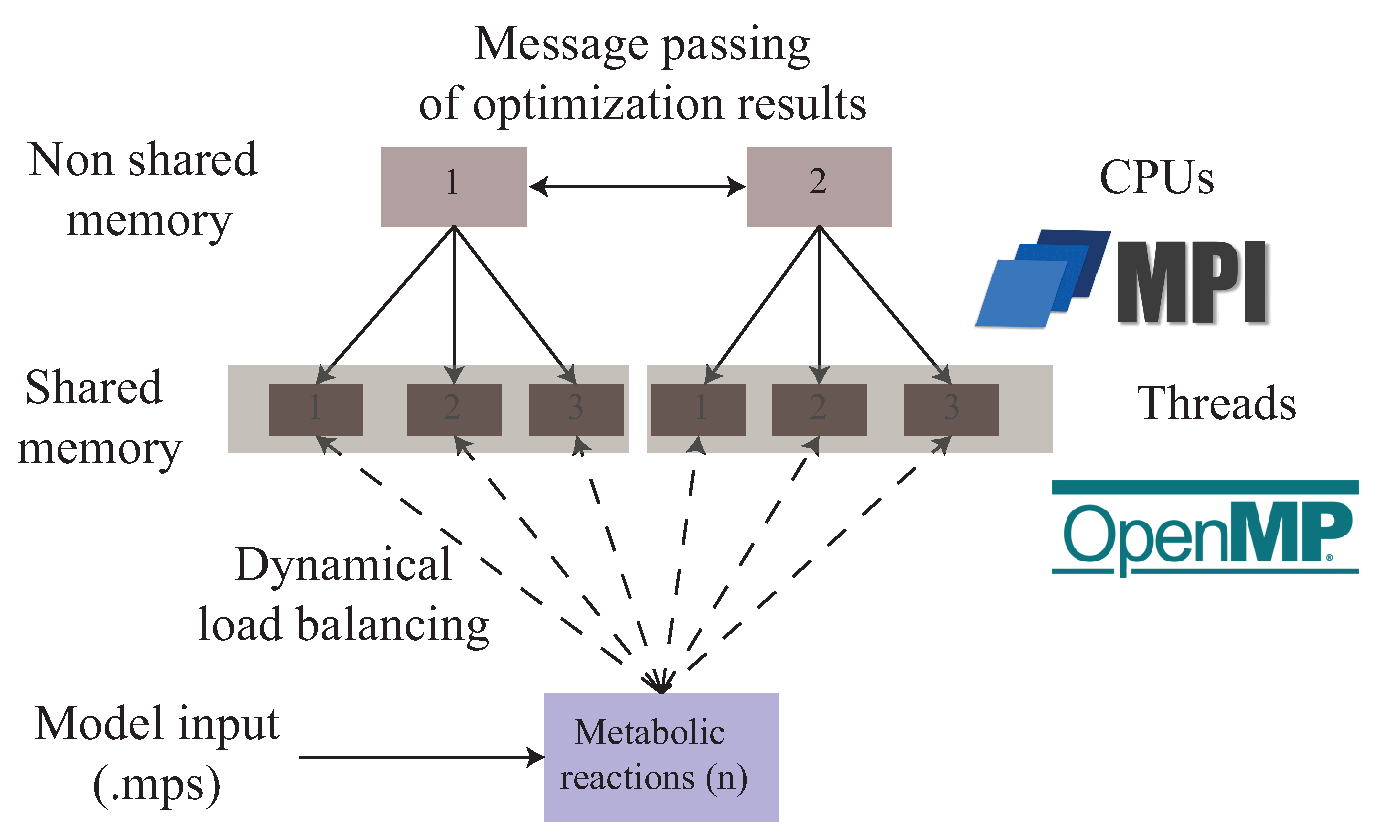
\includegraphics[scale=.3]{figures/figure1/scheme.eps}
\caption{hybrid OpenMP/MPI implementation of FVA.}
\label{fig:hybrid.}
\end{figure}

\subsection{Impact on computing small models}
VFFVA and FFVA were run five times on each model. On small models, VFFVA had at least 20 fold speed-up (the differences between group averages are significant at $p<0.05$) (Table II). The main contributing factor was the use of C over MATLAB in all steps of the analysis. In particular, the loading time of MATLAB java machine and the assignment of workers through \texttt{parpool} was much greater than the analysis time itself.\\
The result highlights the power of C in gaining computing speed, through managing the different low-level aspects of memory allocation and variable declaration.\\
In the analysis of large models, where MATLAB loading time becomes less significant, dynamic load balancing becomes the main driving factor of the gained speed-up.\\ 
\captionof{table}{Comparison of running times of FFVA and VFFVA in small models in seconds.} 
\begin{center}
    \begin{tabular}{ | c | c | c | c |}
    \hline
    Model & \pbox{2cm}{FFVA \\ mean(std) \\ loading and analysis time} & \pbox{2cm}{VFFVA \\ mean(std) \\ loading and analysis time} & \pbox{1.5cm}{FFVA \\ mean(std) \\ analysis only} \\ \hline
    \multicolumn{4}{c}{2 cores} \\ \hline
    Ecoli\textunderscore core & 19.5(0.5)  & 0.2(0.01) & 0.37(0.1) \\ \hline
	Pputida & 19.2(0.7) & 0.6(0.02) & 0.81(0.09) \\ \hline    
    EcoliK12 & 20.4(0.6) & 2.2(0.06) & 2.41(0.09)\\ \hline
        \multicolumn{4}{c}{4 cores} \\ \hline
    Ecoli\textunderscore core & 19.6(0.6)  & 0.2(0.005) & 0.32(0.01) \\ \hline
    Pputida & 19.4(1) &  0.5(0.02) & 0.61(0.01) \\ \hline
    EcoliK12 & 20(0.8) & 1.3(0.04) & 1.64(0.08)\\ \hline
        \multicolumn{4}{c}{8 cores} \\ \hline
    Ecoli\textunderscore core & 19.4(0.5)  & 0.2(0.03) & 0.35(0.05)  \\ \hline
    Pputida & 19.6(0.7) & 0.4(0.04) & 0.53(0.009) \\ \hline
    EcoliK12 & 20(0.49) & 0.9(0.01) & 1.22(0.08)\\ \hline
        \multicolumn{4}{c}{16 cores} \\ \hline
    Ecoli\textunderscore core &  20.2(0.4) & 0.2(0.008) & 0.41(0.05) \\ \hline
    Pputida & 19.5(0.4) & 0.4(0.04) & 0.51(0.03) \\ \hline
    EcoliK12 & 22(0.7) & 0.7(0.01) & 0.87(0.03)\\ \hline
        \multicolumn{4}{c}{32 cores} \\ \hline
    Ecoli\textunderscore core & 22.2(0.4)  & 0.3(0.008) & 0.6(0.12)\\ \hline
    Pputida & 21.5(0.6) &  0.4(0.01) & 0.53(0.004)\\ \hline
    EcoliK12 & 21.5(0.6) & 0.6(0.03) & 0.78(0.04)\\ \hline
    \end{tabular}
\end{center}

\subsection{Impact on computing large models}
The speed-up gained on computing large models (Recon2 and ME) reaches three folds with VFFVA (Fig\ref{fig:largemodel.}). In fact, with dynamic load balancing enabled, VFFVA updates the assigned chunks of iterations to every worker. In this case, faster workers process more iterations, in such way that all workers synchornize at the same time to reduce the results. Particularly, VFFVA increased in speed as the model was bigger and the number of threads rose (Fig\ref{fig:largemodel.}-E\textunderscore Matrix). We explored the different load balancing startegies (static, guided and dynamic) with our largest models (E\textsubscript{c}\textunderscore Matrix and Harvey).

\begin{figure}[!htb]
\centering
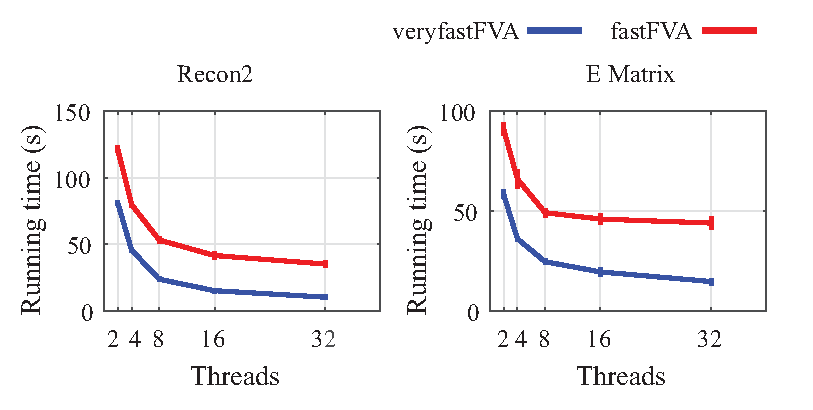
\includegraphics[scale=0.7]{figures/figure2/largemodels.eps}
\caption{Running times of Recon2 and E\textunderscore Matrix model.}
\label{fig:largemodel.}
\end{figure}

\subsection{Load management}
Load management describes the different approaches to assign iterations to the workers. It can be static, where an even number of iterations is assigned to each worker. Guided schedule refers to dividing the iterations in chunks of size $n/workers$ initially and $remaining\textunderscore iterations/workers$ afterwards. The difference with static lies in the dynamic assignment of chunks of the same size, in a way that fast workers can process more iteration blocks. The large scale model simulations (Fig\ref{fig:largemodel.}) used guided scheme. Finally, dynamic schedule is very similar to guided except that chunk size is given by the user, which allows a greater flexibility.

\begin{figure}[!htb]
\centering
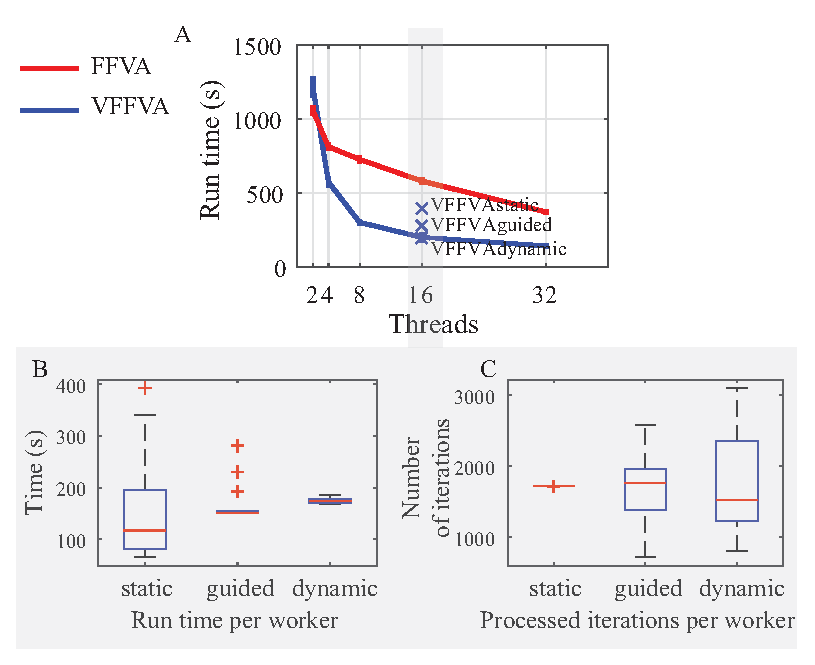
\includegraphics[scale=.7]{figures/figure3/schedule.eps}
\caption{Running times of E\textsubscript{c}\textunderscore Matrix model.}
\label{fig:static.}
\end{figure}

In the following section, we will compare the load balancing strategies of ME\textsubscript{c} model at 16 threads.
\subsubsection{Static schedule}
Using static schedule, VFFVA assigned an equal number of iterations to every worker. With 16 threads, the number of iterations per worker equalled 1715 and 1716 (Fig\ref{fig:static.}-C). Expectedly, the running time varied widely and resulted in a final time of 581$s$.
\subsubsection{Guided schedule}
With guided schedule (Fig\ref{fig:static.}-A), the highest speed-up (2.9) was achieved with 16 threads (Fig\ref{fig:static.}-B). The running time per worker was quite comparable and the iterations processed varied between 719 and 2581.
\subsubsection{Dynamic schedule}
Using a dynamic load balancing with a chunk size of 50 resulted in similar results to the guided schedule. The final running time equalled 197$s$, while FFVA took 581$s$. An optimal chunk size has to be small enough to ensure a frequent update on the workers load, and big enough to take advantage of the solution basis reuse in every worker. At a chunk size of 1 i.e. each worker is assigned 1 iteration at a time, the final solution time equalled 272$s$. The reason being that if the worker is updated quite often with new pieces of iterations, then it looses the stored solution basis of the previous problem and has to solve from scratch. 

\begin{figure}[!htb]
\centering
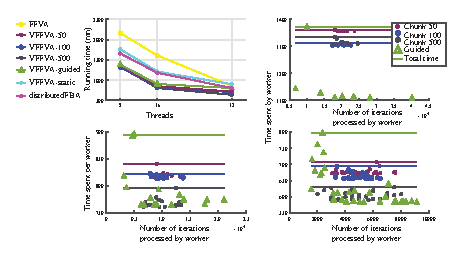
\includegraphics[scale=1.5]{figures/figure4/harvey.eps}
\caption{Running times per worker of Harvey model.}
\label{fig:harvey.}
\end{figure}

Similarly, Harvey model (Fig \ref{fig:harvey.}-A) had a 2-fold speed-up with 16 threads using a chunk size of 50 (821 mn). Running times with guided schedule (1440 mn), dynamic schedule with chunk size 100 (847 mn) and chunk size 500 (1293 mn) were less efficient due to the slower update rate leading to a variable analysis time per worker (Fig \ref{fig:harvey.}-B,C,D). VFFVA on 8 threads (1306 mn with chunk size 50) proved comparable to FFVA (1611 mn) and distributedFBA (1247 mn) both on 16 threads, thereby saving computational resources and time. 

\subsection{Impact on memory usage}

In MATLAB, the execution of $n$ parallel jobs implies launching $n$ instances of MATLAB. On average, one instance needs 2 Gb. In parallel setting, the memory requirements are at minimum $2n$ Gb, which can limit the execution of highly parallel jobs. In the \textit{Julia}-based \texttt{distributedFBA}, the overall memory requirement exceeds 15 Gb at 32 cores. VFFVA requires only the memory necessary to load $n$ instances of the input model. The differences between the FFVA and VFFVA get more pronounced as the number of threads increases (Fig\ref{fig:memory.}) i.e. 13.5 fold at 8 threads, 14.2 fold at 16 threads,14.7 fold at 32 threads.\\
Finally, VFFVA outran FFVA and distributedFBA both on execution time and memory requirements (Table III). The advantage becomes important with larger models and higher number of threads, which makes VFFVA particularly suited for analysing the exponentially-growing-in-size metabolic models in HPC setting.

\begin{center}
\captionof{table}{Comparative summary of the methods' features.} 
    \begin{tabular}{ | c | c | c | c | c |}
    \hline
    Feature & VFFVA & distributedFBA & FFVA & FVA \\ \hline
    Time & ++++ & +++ & ++ & + \\ \hline
    Memory & +++ & ++ & + & + \\ \hline 
    Load balancing & dynamic & static & static & static \\ \hline 
    \end{tabular}
\end{center}

\begin{figure}[!htb]
\centering
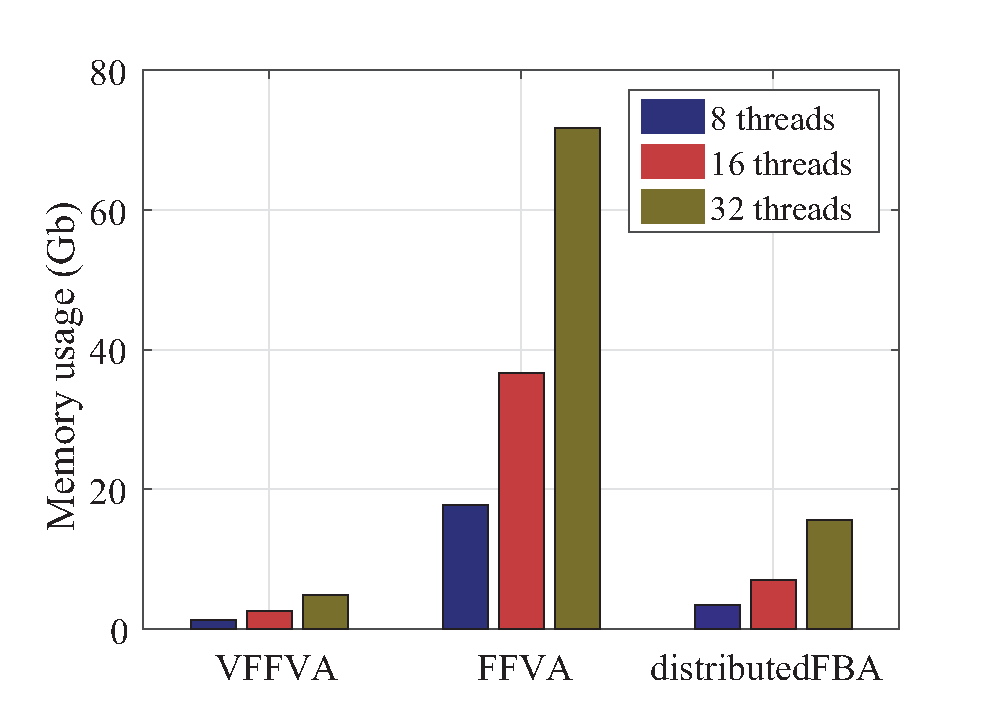
\includegraphics[scale=.5]{figures/figure5/memoryUsage.eps}
\caption{Physical memory usage at 8, 16 and 32 threads.}
\label{fig:memory.}
\end{figure}

\section{Hardware and software}

VFFVA was run on a Dell HPC machine with 72 Intel Xeon E5 2.3GHz cores and 768 GigaBytes of memory. The current implementation was tested with Open MPI v1.10.3, OpenMP 3.1, GCC 4.7.3 and IBM ILOG CPLEX free-of-charge academic version (12.6.3). FFVA was tested with MATLAB 2014b and distributedFBA was run on Julia v0.5. ILOG CPLEX was called with the following parameters:
\begin{equation*} \label{eq:one}
\begin{array}{ll@{}ll}
\texttt{PARALLELMODE=1} &\\
\texttt{THREADS=1} &\\
\texttt{AUXROOTTHREADS=2} &\\
\end{array}
\end{equation*}
Additionally, large scale coupled models with unscaling infeasibilites might require 
\begin{equation*} \label{eq:one}
\begin{array}{ll@{}ll}
\texttt{SCAIND=-1} &\\
\end{array}
\end{equation*}
The call to VFFVA is done from bash as follows:\\
\texttt{mpirun -np \textless nproc\textgreater \hspace{0.1cm}  --bind-to none -x OMP\_NUM\_THREADS=\textless nthr\textgreater \hspace{0.1cm} ./veryfastFVA \textless model.mps\textgreater \hspace{0.1cm} \textless scaling\textgreater}\\
with $nproc$ is the number of non-shared memory processes, $nthr$ is the number of shared memory threads, $scaling$ is CPLEX scaling parameter where 0 leaves it to the default (equilibration) and -1 sets it to unscaling. For large models, OpenMP threads were bound to physical cores through setting the environment variable 
\begin{equation*} \label{eq:one}
\begin{array}{ll@{}ll}
\texttt{OMP\_PROC\_BIND=TRUE} &\\
\end{array}
\end{equation*}
while for small models, setting the variable to \texttt{FALSE}  yielded faster running times.
The schedule is set through the environment variable
\begin{equation*} \label{eq:one}
\begin{array}{ll@{}ll}
\texttt{OMP\_SCHEDULE=<schedule,chunk>} &\\
\end{array}
\end{equation*}
where \texttt{schedule} can be \texttt{static}, \texttt{dynamic} or \texttt{guided}, and \texttt{chunk} is the minimal number of iterations processed per worker at a time. 
Benchamarking was done using $time$ function of bash.
\addtolength{\textheight}{-12cm}   % This command serves to balance the column lengths
                                  % on the last page of the document manually. It shortens
                                  % the textheight of the last page by a suitable amount.
                                  % This command does not take effect until the next page
                                  % so it should come on the page before the last. Make
                                  % sure that you do not shorten the textheight too much.

%%%%%%%%%%%%%%%%%%%%%%%%%%%%%%%%%%%%%%%%%%%%%%%%%%%%%%%%%%%%%%%%%%%%%%%%%%%%%%%%



%%%%%%%%%%%%%%%%%%%%%%%%%%%%%%%%%%%%%%%%%%%%%%%%%%%%%%%%%%%%%%%%%%%%%%%%%%%%%%%%



%%%%%%%%%%%%%%%%%%%%%%%%%%%%%%%%%%%%%%%%%%%%%%%%%%%%%%%%%%%%%%%%%%%%%%%%%%%%%%%%

\section*{ACKNOWLEDGMENT}

The authors would like to acknowledge fastFVA authors for publicly sharing their code, IBM for providing a free academic version of ILOG CPLEX as well as Valentin Plugaru and Dr. Laurent Heirendt at the University of Luxembourg, for useful comments and guidance. The experiments presented in this paper were carried out
in part using the HPC facilities of the University of Luxembourg~\cite{VBCG_HPCS14} 
{\small -- see \url{http://hpc.uni.lu}}.



%%%%%%%%%%%%%%%%%%%%%%%%%%%%%%%%%%%%%%%%%%%%%%%%%%%%%%%%%%%%%%%%%%%%%%%%%%%%%%%%

\bibliography{refExtr} 
\bibliographystyle{ieeetr}



\end{document}
